% This file was created with tikzplotlib v0.10.1.
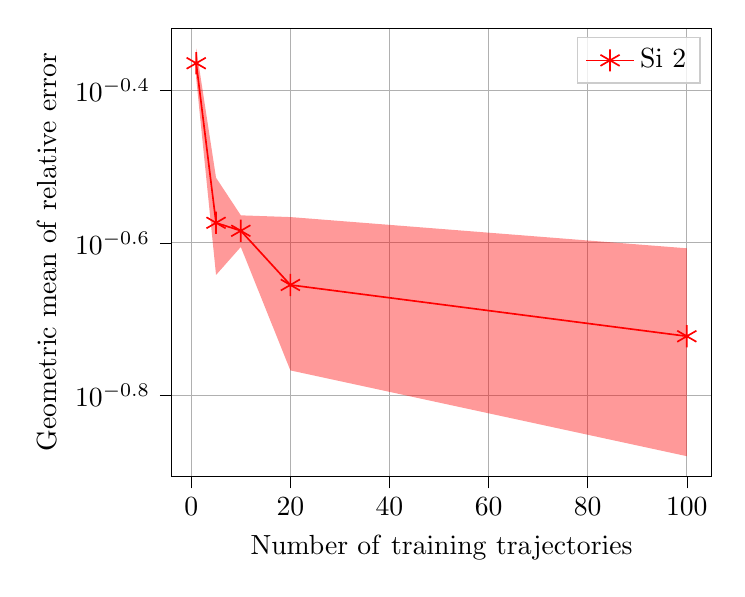
\begin{tikzpicture}

\definecolor{darkgray176}{RGB}{176,176,176}
\definecolor{lightgray204}{RGB}{204,204,204}

\begin{axis}[
legend cell align={left},
legend style={fill opacity=0.8, draw opacity=1, text opacity=1, draw=lightgray204},
log basis y={10},
tick align=outside,
tick pos=left,
x grid style={darkgray176},
xlabel={\(\displaystyle \mathrm{Number \ of \ training \ trajectories }\)},
xmajorgrids,
xmin=-3.95, xmax=104.95,
xtick style={color=black},
y grid style={darkgray176},
ylabel={\(\displaystyle \mathrm{Geometric \ mean \ of \ relative \ error }\)},
ymajorgrids,
ymin=0.124202278932207, ymax=0.479868063422627,
ymode=log,
ytick style={color=black}
]
\path [fill=red, fill opacity=0.4, semithick]
(axis cs:1,0.451274070095849)
--(axis cs:1,0.412334431390405)
--(axis cs:5,0.228066082459979)
--(axis cs:10,0.24816016186378)
--(axis cs:20,0.171047418830359)
--(axis cs:100,0.132072084379269)
--(axis cs:100,0.247162499016812)
--(axis cs:100,0.247162499016812)
--(axis cs:20,0.271568947065038)
--(axis cs:10,0.272977439391823)
--(axis cs:5,0.305772372928571)
--(axis cs:1,0.451274070095849)
--cycle;

\addplot [semithick, red, mark=asterisk, mark size=4, mark options={solid}]
table {%
1 0.431804269552231
5 0.266919195652008
10 0.260568797588348
20 0.221308141946793
100 0.189617291092873
};
\addlegendentry{Si 2}
\end{axis}

\end{tikzpicture}
